\documentclass[a4paper,11pt]{article}
\usepackage[T1]{fontenc}
\usepackage[utf8]{inputenc}
\usepackage{lmodern}
\usepackage{upgreek}
\usepackage{amsmath}
\usepackage{mathabx}
\usepackage{MnSymbol}
\usepackage{wasysym}
\usepackage{booktabs}
\usepackage{graphicx}
\usepackage[]{algorithm2e}
\usepackage{hyperref}
\usepackage{tikz}
\usepackage[czech]{babel}
\usepackage{rotating}
\usepackage{placeins}
\usepackage{listings}
\usepackage{dipp8}
\usetikzlibrary{arrows,automata,positioning}

\author{Martin Hnátek}
\title{Dokumentace k samostatnému projektu do TPJ\\Programovací jazyk Mirage}

\date{}

\begin{document}

\maketitle

\newpage
\tableofcontents

\newpage

\section{Zadání}
Cílem projektu bylo vytvořit programovací jazyk jehož programy popisují obrázek ve vektorovém formátu svg. Toto umožňuje tvorbu obrázků jejichž parametry lze volně měnit, což je užitečné například pro tvorbu fraktálních obrazců.

\section{Popis jazyka}
Mirage je inspirován rodinou programovacích jazyků typu lisp. Z tohoto plyne jak dosti specifická syntaxe, tak i pokročilejší možnosti, jako je například metaprogramování s pomocí maker. Následující sekce slouží jako přehled pro vlastnosti Mirage.

\subsection{Datové typy}
Mirage má následující datové typy:
\begin{enumerate}
	\item číslo - Implementuje číslo v rozsahu doporučeném standardem svg. Tedy float
	\item řetězec - Řetězec začíná a končí " je možné uvnitř něj escapovat jakýkoliv znak
	\item logická hodnota - Logický datový typ má 2 možné hodnoty pravda - \$p nebo nepravda \$n
	\item funkce
	\item makro
	\item list
	\item SVG element - Tisknutelný popis svg elementu
\end{enumerate}

\subsection{Funkce}
Každá funkce v Mirage má seznam argumentů a tělo obsahující alespoň jeden výraz. Poslední výraz v těle je návratová hodnota. Když se v seznamu argumentů objeví identifikátor ... je funkce variadická a do tohoto identifikátoru je vložen list 0 až nekonečno hodnot v závislosti na počtu argumentů. Argument ... musí být v seznamu argumentů poslední.

\begin{lstlisting}[language=lisp]
; Ukazka funkce
((funkce (x) x) 5) ; Vrati 5
((funkce (...) (prvni ...)) 1 2 3) ; Vrati 1
\end{lstlisting}

Poslední věcí, která je potřeba zmínit je rekurze. Rekurzivní volání bývá v klasických jazycích problematické, protože rychle dochází k přetečení stacku. Mirage a ostatní lispy tento problém řeší s pomocí optimalizace, která se nazývá tail call eleminace. Tato optimalizace říká, že pokud máme funkci, která vrací volání sama sebe lze jí optimalizovat tak, že se vrátíme na začátek funkce a jen zaměníme její argumenty za voláné hodnoty. Příklad tohoto chování je níže:

\begin{lstlisting}[language=lisp]
(definuj faktorial (funkce (x akumulator)
	(pokud (= x 0)
		akumulator
		(faktorial (- x 1) (* x akumulator)))))
\end{lstlisting}

Pokaždé, když program dojde na volání faktorialu, tak se promění argument x za (- x 1) a akumulator za (* x akumulator) a funkce se vyhodnocuje znovu s novými hodnotami. Tato optimalizace ovšem funguje pouze, když je volání funkce na posledním místě. Například níže uvedený kód spustí klasickou rekurzi

\begin{lstlisting}[language=lisp]
(definuj faktorial (funkce (x)
	(pokud (= x 0)
		1
		(* x (faktorial (- x 1))))))
\end{lstlisting}

\subsection{Makra}
Makra jsou funkce, které nevyhodnocují své argumenty a jejíchž návratová hodnota je list, který se evaluuje jako normální kód v Mirage. K makrům se váží 2 funkce nevyhodnocuj a vyhodnot.

Funkce nevyhodnocuj bere jakoukoliv validní hodnotu a vrací její nevyhodnocenou podobu. Pokud je to identifikátor vrátí nevyhodnocený identifikátor, pokud je to hodnotový datový typ (řetězec, číslo, ...), tak jej vrátí nezměněný. Pokud se jedná o výraz, tak jej převede na list nevyhodnocených hodnot. Příklad:

\begin{lstlisting}[language=lisp]
; Ukazka funkce
(nevyhodnot (+ 5 6)) ; Vrati (list (nevyhodnot +) 5 6)
(nevyhodnot +) ; Vrati identifikator +
\end{lstlisting}

Funkce vyhodnot je inverzní funkcí k funkci nevyhodnocuj. Například

\begin{lstlisting}[language=lisp]
; Ukazka funkce
(vyhodnot (list + 5 6)) ; Vrati 11
(vyhodnot (nevyhodnocuj +)) ; Vrati funkci +
\end{lstlisting}

Makro si můžeme představit jako funkci, která na každý svůj argument zavolá nevyhodnocuj a pak na svůj výstup zavolá vyhodnoť. Příkladem užitečného makra je makro aplikuj, které se nachází ve standardní knihovně jazyka Mirage. Aplikuj bere funkci a list hodnot a vygeneruje kód, který volá funkci s hodnotami v listu. Její implementace je zde

\begin{lstlisting}[language=lisp]
(definuj aplikuj ; definice
	(makro (fn argumenty)
		(spoj (list fn) argumenty)))
		
; Prelozi se do (+ 5 6), coz se vyhodnoti do 11
(aplikuj + (list 5 6)) 
\end{lstlisting}

Makra se rozbalují a vyhodnocuje ve scopu toho, kdo je volá, což umožňuje například tail call eliminace. Například makro pokud (ukázka výše u funkce faktorial) vyhodnotí svůj první argument a pak se rozbalí do prvního nebo druhého argumentu na základě toho, jestli je pravda nebo nepravda.

\begin{lstlisting}[language=lisp]
; V tomto pripade se makro rozbali do (+ 1 2)
; a volani chyby se vubec nevyhodnoti
(pokud $p
	(+ 1 2)
	(chyba "Kriticka chyba!"))
\end{lstlisting}

\subsection{Expanze}
Expanze jsou syntaktický cukr pro volání funkcí, který vychází ze skutečnosti, že pokud má funkce pouze jeden vstupní argument, tak jí není třeba obalovat do závorek. Například výše uvedená funkce nevyhodnocuj přebírá pouze jeden argument, takže jí lze s pomocí expanzí zapsat následujícím způsobem:
\begin{lstlisting}[language=lisp]
; Vrati (list (nevyhodnocuj +) 1 2)
; Je ekvivalentni k (#nevyhodnocuj (+ 1 2))
#nevyhodnocuj (+ 1 2) 
\end{lstlisting}
Jelikož parser očekává za názvem expanze nějáký platný výraz není možné jí vytvořit s pomocí funkce definuj. Proto existuje funkce definujExpanzi, která se chová úplně stejně jako definuj s tím rozdílem, že před identifikátor přidá \#. Ve standardní knihovně se nachází makro funkce->expanze, které přebírá jakoukoliv funkci nebo makro a vygeneruje expanzi, která přebírá libovolný počet argumentů její použití je následujíci.
\begin{lstlisting}[language=lisp]
#importuj "mirage/mirage.mir"
(funkce->expanze + plus)
#plus (1 2 3) ; Vrati 6
\end{lstlisting}

\subsection{Standardní knihovna}
Mirage obsahuje malou standardní knihovnu, která zahrnuje spoustu užitečných definic včetně funkcí, které generují samotné SVG elementy. Pro její použití je nutné jí naimportovat a mít správně nastavenou proměnnou prostředí MIRAGE\_PATH (více v sekci spuštění). Jako jeden příklad za všechny si dovolím uvést použití makra defn, které zjednodušuje definici funkcí.

\begin{lstlisting}[language=lisp]
(importuj "mirage/mirage.mir")

(defn faktorial (x)
	(pokud (= x 0)
		1
		(* x (faktorial (- x 1)))))
\end{lstlisting}


\subsection{Kreslení}
Jak již bylo řečeno, jazyk Mirage je jazyk pro generování obrázku ve formátu svg. Samotné kreslení je založeno na dvou funkcích element a vykresli. Funkce element reprezentuje svg element. Funkce přebírá název elemntu jeho argumenty (list řetězců) a jeho následníky (list potomků).

Příkladem použití funkce element může být funkce obdelnik, ktera vraci reprezentaci obdelniku.

\begin{lstlisting}[language=lisp]
(definuj obdelnik (funkce (vyska sirka)
	 (element "rect" 
	 	(list "width" (hodnota->retezec sirka) 
	 	      "height" (hodnota->retezec vyska)) 
	 	(list))))
\end{lstlisting}
Funkce vykresli přebírá seznam elementů, výšku a šířku výsledného svg obrázku. Při jejím zavolání se celý obrázek vypíše na stdout a program je následně ukončen. Příklad vykreslení obdelníku:

\begin{lstlisting}[language=lisp]
(importuj "mirage/mirage.mir")

(vykresli (list (obdelnik 100 100)) 100 100)
\end{lstlisting}
\definecolor{maroon}{rgb}{0.5,0,0}
\definecolor{darkgreen}{rgb}{0,0.5,0}
\lstdefinelanguage{XML}
{
  basicstyle=\ttfamily,
  morestring=[s]{"}{"},
  morecomment=[s]{?}{?},
  morecomment=[s]{!--}{--},
  commentstyle=\color{darkgreen},
  moredelim=[s][\color{black}]{>}{<},
  moredelim=[s][\color{red}]{\ }{=},
  stringstyle=\color{blue},
  identifierstyle=\color{maroon}
}
Vypíše 
\begin{lstlisting}[language=XML]
<svg width="100"
     height="100"
     xmlns="http://www.w3.org/2000/svg">     
	<rect height="100"
	      width="100"></rect>
</svg>
\end{lstlisting}

\section{Lexikální analýza}
V této sekci se nachází popis jednotlivých gramatik, které jsou zpracovány lexikálním analyzátorem.

\subsection{Identifikátory}
Identifikátor začíná na kterýkoliv znak z množiny $z = \{a..z, A..Z, +, -, /, *, <\}$
a pokračuje v libovolném znaku z množiny $m = z \bigcup \{0..9\}$ 
\linebreak

$G_{identifikatory}$(\{S, A, B\}, \{z, m\}, P, S)
$$S \rightarrow zA | z$$
$$A \rightarrow mA | m$$

\subsection{Čísla}
$G_{cisla}$(\{S, B, C\}, \{d, .\}, P, S)
$$S \rightarrow dB | d$$
$$B \rightarrow dB | d | .C$$
$$C \rightarrow dC | d$$

\subsection{Řetězce}
Řetězce začínají a končí na znak ". V samotném řetězci se pak může nacházet jakýkýkoliv znak před kterým se nachází $\backslash$ nebo cokoliv v množině $\blacksquare$, která reprezentuje všechny tisknutelné znaky, které nejsou $\backslash$ nebo ".

$G_{retezce}$(\{S, D, E\}, \{$\backslash, ", \blacksquare$\}, P, S)
$$S \rightarrow "D$$
$$D \rightarrow " | \backslash E | \blacksquare E$$
$$E \rightarrow "D | \backslash D | \blacksquare D$$

\subsection{Závorky}
Závorky hrají v lispu důležitou roli. Rozhodl jsem se, že pro jednoduchost bude jazyk podporovat jen \textquotedblleft kulaté \textquotedblright závorky
$G_{zavorky}$(\{S\}, \{(, )\}, P, S)

$$S \rightarrow (|)$$

\subsection{Gramatika bílých znaků}
Je gramatika popisující všechny bílé znaky $G_{bileznaky}$(\{S\}, \{$\dlsh | \mapsto | \sqcup$\}, P, S)
$$S \rightarrow  \dlsh S | \mapsto S | \sqcup S$$

\subsection{Komentáře}
Jazyk má jednoduché komentáře začínající na ; nebo \# a končící novým řádkem $G_{komentare}$(\{S, F\}, \{$\dlsh$, ;, $\Square$\}, P, S)

$$S \rightarrow ;F $$
$$F \rightarrow \Square F | \dlsh S$$

\subsection{Symboly pro expanzi parserem}

$G_{expanze}$(\{S, G\}, \{ $\boxplus$, \# \})

$$S \rightarrow \#G$$
$$G \rightarrow \boxplus G | \boxplus$$

Kde $\boxplus$ je množina všech nebilých znaků včetně \#. 

\subsection{Logické hodnoty}
Logická hodnota může být buď \$p pro pravdu (true) a \$n pro nepravdu:
\\
$G_{logicke}$(\{S, H\}, \{\$, n, p\})

$$S \rightarrow \$H$$
$$H \rightarrow n | p$$

\section{Stavový automat}
Nyní je třeba z předem definované gramatiky spojit a převést na automat. Pokud tento automat nebude deterministický je třeba jej determinizovat.

Samotný jazyk se skládá z jazyku oddělovačů (komentáře, bílé znaky) $L_{od} = G_{komentare} \bigcup G_{bileznaky}$ a jazyku významových tokenů. 

$$L_{vt} = L_{identifikatory} \bigcup L_{cisla} \bigcup L_{retezce} \bigcup L_{zavorky}$$
Celý jazyk pak lze zapsat tímto způsobem 
$$L = (L^{*}_{od}.L_{vt})^{*}.L^{*}_{od}$$
Po spojení nám vzniká gramatika
 
%%% Gramatika
$G_{vt}$(\{S, $S_{identifikatory}$, $S_{cisla}$, $S_{retezce}$, $S_{zavorky}$, A, B, C, D, E, F, G\}, \{d, z, m, (, ), $\backslash$ \}, P, S), která reprezentuje významové tokeny 

$$S \rightarrow S_{identifikatory} | S_{cisla} | S_{retezce} | S_{zavorky} | S_{od}$$

kde neterminál $S_{od}$ je definovaný v gramatice oddělovačů $G_{od}$(\{S, A\}, \{$\mapsto$, $\sqcup$, $\dlsh$, ;\}, P, S)

$$S \rightarrow \dlsh | \mapsto | \sqcup | ;A | \Square$$
$$A \rightarrow \Square A | ;A | \dlsh $$

Po spojení gramatik a odstranění jednoduchých pravidel dostaváme gramatiku
$G_{finalni}$(\{$S, A, B, C, D, E, F, G, H$\}, \{$\mapsto$, $\sqcup$, $\dlsh$, ;, $\Square$, $\backslash$, $\blacksquare$, $\boxplus$, ", d, ., z, m, (, ), \$, \#, p, n\}, P, S)
$$S \rightarrow zA | z | dB | d | "D | ;F | \dlsh S | \mapsto S | \sqcup S | ( | ) | \#G | \$H$$
$$A \rightarrow mA | m$$
$$B \rightarrow dB | d | .C$$
$$C \rightarrow dC | d$$
$$D \rightarrow " | \backslash E | \blacksquare D$$
$$E \rightarrow "D | \backslash D | \blacksquare D$$
$$F \rightarrow \Square F | \dlsh S$$
$$G \rightarrow \boxplus G | \boxplus$$
$$H \rightarrow n | p$$

\begin{sidewaystable}[]
%\centering
	\begin{tabular}{@{}lcccccccccccccccccc@{}}
		\toprule
		\multicolumn{1}{c}{$\delta$} & z & m & d & . & $\backslash$ & “ & ( & ) & $\dlsh$ & $\mapsto$ & $\sqcup$ & ; & $\Square$ & $\boxplus$ & \$ & \# & p & n \\ \midrule
		$Q_{S}$ & $Q_{A\hat{F}}$ & - & $Q_{B, \hat{F}}$ & - & - & $Q_{D}$ & $Q_{\hat{F}}$ & $Q_{\hat{F}}$ & $Q_{S}$ & $Q_{S}$ & $Q_{S}$ & $Q_{F}$ & - & - & $Q_{H}$ & $Q_{G}$ & - & - \\
		$Q_{C}$ & $Q_{C, \hat{F}}$ & - & - & - & - & - & - & - & - & - & - & - & - & - & - & - & - & - \\
		$Q_{D}$ & - & - & - & - & - & $Q_{D}$ & - & $Q_{E}$ & - & - & $Q_{\hat{F}}$ & - & - & - & - & - & - & - \\
		$Q_{E}$ & - & - & - & - & - & $Q_{D}$ & - & $Q_{D}$ & - & - & $Q_{D}$ & - & - & - & - & - & - & - \\
		$Q_{F}$ & - & - & - & - &  & - & $Q_{F}$ & - & - & - & - & $Q_{S}$ & - & - & - & - & - & - \\
		$Q_{G}$ & - & - & - & - & - & - & - & - & - & - & - & - & - & $Q_{G, \hat{F}}$ &  &  & - & - \\
		$Q_{H}$ & - & - & - & - & - & - & - & - & - & - & - & - & - & - & - & - & $Q_{\hat{F}}$ & $Q_{\hat{F}}$ \\
		$Q_{\hat{F}}$ & - & - & - & - & - & - & - & - & - & - & - & - & - & - & - & - & - & - \\
		$Q_{A,\hat{F}}$ & - & - & $Q_{A\hat{F}}$ & - & - & - & - & - & - & - & - & - & - & - & - & - & - & - \\
		$Q_{B, \hat{F}}$ & $Q_{B, \hat{F}}$ & - & - & - & - & - & - & - & - & $Q_{C}$ & - & - & - & - & - & - & - & - \\
		$Q_{C, \hat{F}}$ & $Q_{C, \hat{F}}$ & - & - & - & - & - & - & - & - & - & - & - & - & - & - & - & - & - \\
		$Q_{G, \hat{F}}$ & - & - & - & - & - & - & - & - & - & - & - & - & - & $Q_{G, \hat{F}}$ & - & - & - & - \\ \bottomrule
		\end{tabular}
		\caption{Tabulka popisující DFA}
	\label{Tabulka popisující DFA}
\end{sidewaystable}

%\newpage

\begin{center}
\begin{tikzpicture}[scale=0.2]
\tikzstyle{every node}+=[inner sep=0pt]
\draw [black] (8,-28.2) circle (3);
\draw (8,-28.2) node {$Q_{S}$};
\draw [black] (26.4,-6.4) circle (3);
\draw (26.4,-6.4) node {$Q_{B\hat{F}}$};
\draw [black] (26.4,-6.4) circle (2.4);
\draw [black] (64.6,-13.4) circle (3);
\draw (64.6,-13.4) node {$Q_{A\hat{F}}$};
\draw [black] (64.6,-13.4) circle (2.4);
\draw [black] (72.9,-40.5) circle (3);
\draw (72.9,-40.5) node {$Q_{\hat{F}}$};
\draw [black] (72.9,-40.5) circle (2.4);
\draw [black] (59.4,-6.4) circle (3);
\draw (59.4,-6.4) node {$Q_{C\hat{F}}$};
\draw [black] (59.4,-6.4) circle (2.4);
\draw [black] (12.9,-47.7) circle (3);
\draw (12.9,-47.7) node {$Q_{D}$};
\draw [black] (66,-24.7) circle (3);
\draw (66,-24.7) node {$Q_{F}$};
\draw [black] (61.1,-55.6) circle (3);
\draw (61.1,-55.6) node {$Q_{E}$};
\draw [black] (40.1,-6.4) circle (3);
\draw (40.1,-6.4) node {$Q_{C}$};
\draw [black] (22.3,-37.6) circle (3);
\draw (22.3,-37.6) node {$Q_{H}$};
\draw [black] (8,-17) circle (3);
\draw (8,-17) node {$Q_{G}$};
\draw [black] (10.5,-7.5) circle (3);
\draw (10.5,-7.5) node {$Q_{G,\hat{F}}$};
\draw [black] (9.93,-25.91) -- (24.47,-8.69);
\fill [black] (24.47,-8.69) -- (23.57,-8.98) -- (24.33,-9.63);
\draw (17.75,-18.74) node [right] {$d$};
\draw [black] (10.9,-27.44) -- (61.7,-14.16);
\fill [black] (61.7,-14.16) -- (60.8,-13.88) -- (61.05,-14.85);
\draw (37.09,-21.37) node [below] {$z$};
\draw [black] (10.95,-28.76) -- (69.95,-39.94);
\fill [black] (69.95,-39.94) -- (69.26,-39.3) -- (69.07,-40.28);
\draw (41.29,-33.71) node [above] {$(,)$};
\draw [black] (65.49,-10.547) arc (190.39718:-97.60282:2.25);
\draw (70.72,-8.03) node [above] {$m$};
\fill [black] (67.41,-12.37) -- (68.28,-12.72) -- (68.1,-11.74);
\draw [black] (58.077,-3.72) arc (234:-54:2.25);
\draw (59.4,0.85) node [above] {$d$};
\fill [black] (60.72,-3.72) -- (61.6,-3.37) -- (60.79,-2.78);
\draw [black] (8.73,-31.11) -- (12.17,-44.79);
\fill [black] (12.17,-44.79) -- (12.46,-43.89) -- (11.49,-44.14);
\draw (9.69,-38.41) node [left] {$"$};
\draw [black] (63.16,-25.667) arc (-72.01092:-101.08244:104.23);
\fill [black] (63.16,-25.67) -- (62.25,-25.44) -- (62.55,-26.39);
\draw (37.31,-31.12) node [below] {$;$};
\draw [black] (58.103,-55.466) arc (-93.00582:-105.61026:195.334);
\fill [black] (58.1,-55.47) -- (57.33,-54.92) -- (57.28,-55.92);
\draw (34.28,-54.21) node [below] {$\backslash$};
\draw [black] (15.88,-47.34) -- (69.92,-40.86);
\fill [black] (69.92,-40.86) -- (69.07,-40.46) -- (69.19,-41.45);
\draw (43.15,-44.68) node [below] {$"$};
\draw [black] (15.899,-47.753) arc (88.44043:72.94349:159.117);
\fill [black] (15.9,-47.75) -- (16.69,-48.27) -- (16.71,-47.28);
\draw (43.03,-48.03) node [above] {$\blacksquare,\backslash,"$};
\draw [black] (67.745,-22.274) arc (172.01431:-115.98569:2.25);
\draw (72.64,-20.37) node [right] {$\Square$};
\fill [black] (68.99,-24.61) -- (69.71,-25.22) -- (69.85,-24.22);
\draw [black] (5.32,-29.523) arc (-36:-324:2.25);
\draw (0.75,-28.2) node [left] {$\dlsh,\mbox{ }\mapsto,\mbox{ }\sqcup$};
\fill [black] (5.32,-26.88) -- (4.97,-26) -- (4.38,-26.81);
\draw [black] (63.01,-24.88) -- (10.99,-28.02);
\fill [black] (10.99,-28.02) -- (11.82,-28.47) -- (11.76,-27.47);
\draw (36.78,-25.79) node [above] {$\dlsh$};
\draw [black] (13.882,-50.522) arc (46.9079:-241.0921:2.25);
\draw (10.12,-55.53) node [below] {$\blacksquare$};
\fill [black] (11.26,-50.2) -- (10.35,-50.44) -- (11.08,-51.12);
\draw [black] (23.581,-7.392) arc (317.11154:29.11154:2.25);
\draw (19.03,-5.47) node [left] {$d$};
\fill [black] (23.9,-4.77) -- (23.65,-3.85) -- (22.97,-4.59);
\draw [black] (29.4,-6.4) -- (37.1,-6.4);
\fill [black] (37.1,-6.4) -- (36.3,-5.9) -- (36.3,-6.9);
\draw (33.25,-6.9) node [below] {$.$};
\draw [black] (43.1,-6.4) -- (56.4,-6.4);
\fill [black] (56.4,-6.4) -- (55.6,-5.9) -- (55.6,-6.9);
\draw (49.75,-6.9) node [below] {$d$};
\draw [black] (10.51,-29.85) -- (19.79,-35.95);
\fill [black] (19.79,-35.95) -- (19.4,-35.09) -- (18.85,-35.93);
\draw (13.65,-33.4) node [below] {$\$$};
\draw [black] (25.3,-37.77) -- (69.9,-40.33);
\fill [black] (69.9,-40.33) -- (69.13,-39.78) -- (69.08,-40.78);
\draw (47.46,-39.66) node [below] {$p,n$};
\draw [black] (8,-25.2) -- (8,-20);
\fill [black] (8,-20) -- (7.5,-20.8) -- (8.5,-20.8);
\draw (8.5,-22.6) node [right] {$\#$};
\draw [black] (8.76,-14.1) -- (9.74,-10.4);
\fill [black] (9.74,-10.4) -- (9.05,-11.05) -- (10.02,-11.3);
\draw (10.01,-12.75) node [right] {$\boxplus$};
\draw [black] (7.623,-6.69) arc (282.01279:-5.98721:2.25);
\draw (4.94,-1.53) node [left] {$\boxplus$};
\fill [black] (9.39,-4.72) -- (9.72,-3.84) -- (8.74,-4.05);
\end{tikzpicture}
\end{center}

\section{Parsování}
Návrh gramatiky pro parser vychází z následujících syntaktických diagramů.
\newpage
\subsection{Program}
Každý program se skládá z 0 až $\infty$ výrazů.

\begin{figure}[!h]
	%\FloatBarrier
    \centering
    
\includegraphics[width=0.3\textwidth]{obrazky/Program.png}
    \caption{Syntaktický diagram pro program}
    \label{fig:Syntaktický diagram pro program}
\end{figure}

\subsection{Vyraz}
Výraz může být buď tzv. s-expression, což je ozávorkovaný list argumentů.

\begin{figure}[!h]
	%\FloatBarrier
    \centering
    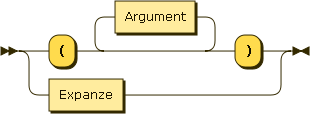
\includegraphics[width=0.5\textwidth]{obrazky/Vyraz.png}
    \caption{Syntaktický diagram pro Atom}
    \label{fig:Syntaktický diagram pro Atom}
\end{figure}
\subsection{Atom}
Atom představuje základní element jazyka Mirage. Může to být buď řetězec, číslo nebo identifikátor.
\begin{figure}[!h]
	%\FloatBarrier
    \centering
    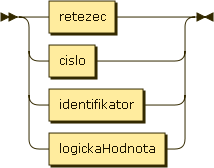
\includegraphics[width=0.5\textwidth]{obrazky/Atom.png}
    \caption{Syntaktický diagram pro Atom}
    \label{fig:Syntaktický diagram pro Atom}
\end{figure}

\newpage

\subsection{Argument}
Je element, který se nachází buď v s-expressionu nebo v expanzi.
\begin{figure}[!h]
	%\FloatBarrier
    \centering
    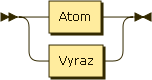
\includegraphics[width=0.3\textwidth]{obrazky/Argument.png}
    \caption{Syntaktický diagram pro Atom}
    \label{fig:Syntaktický diagram pro Atom}
\end{figure}

\subsection{Expanze}
\begin{figure}[!h]
	%\FloatBarrier
    \centering
    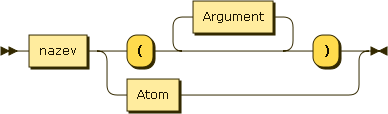
\includegraphics[width=0.65\textwidth]{obrazky/Expanze.png}
    \caption{Syntaktický diagram pro Atom}
    \label{fig:Syntaktický diagram pro Atom}
\end{figure}

\subsection{Parsovací algoritmus}
Pro samotné parsování je použit algoritmus přepisu rozkladové tabulky. Výše uvedená gramatika je obohacena o sémantické akce, které jí říkají, kdy má sestavit sémantický strom a kdy ho má vyhodnotit.

\section{Gramatika pro parsování}
Z výše uvedených syntaktických diagramů vychází následující gramatika pro syntaktický analyzátor.
$$G_syntaktickyAnalyzator({Program, Vyraz, Vyraz2, Argument, Expanze, Atom},$$
$${(, ), nazev, cislo, identifikator, retezec, logickaHodnota},
P,
Program)$$
$$Program \rightarrow Vyraz\:Program\:|\:\epsilon$$
$$Vyraz \rightarrow\:(\:Vyraz2\:|\:Expanze$$
$$Vyraz2 \rightarrow\:Argument\:Vyraz2\:|\:)$$
$$Argument \rightarrow Atom\:|\:Vyraz$$
$$Expanze \rightarrow nazev\:Argument$$
$$Atom \rightarrow cislo | identifikator | retezec | logickaHodnota$$

\section{Gramatika obohacená o sémantické akce}
Následující gramatika byla doplněna o dvě sémantické akce Volani, které vyhodnotí aktualní strom a SestavStrom, která "uzavře" sémantický strom a přesune ho o úroveň nahoru.
$$G_syntaktickyAnalyzator({Program, Vyraz, Vyraz2, Argument, Expanze, Atom},$$
$${(, ), nazev, cislo, identifikator, retezec, logickaHodnota},
P,
Program)$$
$$Program \rightarrow Vyraz\:Program\:Volani\:|\:\epsilon$$
$$Vyraz \rightarrow\:(\:Vyraz2\:|\:Expanze$$
$$Vyraz2 \rightarrow\:Argument\:Vyraz2\:|\:)\:SestavStrom$$
$$Argument \rightarrow Atom\:|\:Vyraz$$
$$Expanze \rightarrow nazev\:Argument\:SestavStrom$$
$$Atom \rightarrow cislo | identifikator | retezec | logickaHodnota$$

\subsection{Množiny first a follow a parsovací tabulka}
Pro tvorbu parsovací tabulky je třeba spočítat množiny first a follow, které vychází z popsané gramatiky.

$$First(Program) = \{\$, (, nazev\}$$
$$First(Vyraz) =  \{(,nazev\}$$
$$First(Vyraz2) = \{),(,cislo,identifikator,rtezec,logickaHodnota,nazev\}$$
$$First(Expanze) = \{ nazev \}$$
$$First(Argument) = \{(,cislo,identifikator,rtezec,logickaHodnota,nazev\}$$
$$First(Atom) = \{cislo, identifikator, retezec, logickaHodnota\}$$

$$Follow(Program) = \{\$, Volani\}$$
$$Follow(Vyraz) = \{\$,(,nazev,Volani,),cislo,identifikator,retezec,logickaHodnota,SestavStrom\}$$
$$Follow(Vyraz2) = \{\$,(,nazev,Volani,),cislo,identifikator,retezec,logickaHodnota,SestavStrom\}$$
$$Follow(Expanze) = \{\$,(,nazev,Volani,),cislo,identifikator,retezec,logickaHodnota,SestavStrom\}$$
$$Follow(Argument) = \{),(,cislo,identifikator,rtezec,logickaHodnota,nazev,SestavStrom\}$$

Z toho lze vyvodit následující tabulku:
% Please add the following required packages to your document preamble:
% \usepackage{booktabs}
\begin{sidewaystable}[]
\centering
\resizebox{\textwidth}{!}{%
\begin{tabular}{@{}llllllllll@{}}
\toprule
 & Volani & ( & ) & nazev & cislo & identifikator & rtezec & logickaHodnota & \$ \\ \midrule
Program &   $\epsilon$ &   Vyraz Program Volani &  &   Vyraz Program Volani &  &  &  &  &   '' \\
Vyraz &  &   ( Vyraz2 &  &   Expanze &  &  &  &  &  \\
Vyraz2 &  &   Argument Vyraz2 &   ) SestavStrom &   Argument Vyraz2 &   Argument Vyraz2 &   Argument Vyraz2 &   Argument Vyraz2 &   Argument Vyraz2 &  \\
Argument &  & Vyraz &  & Vyraz & Atom & Atom & Atom &   Atom &  \\
Expanze &  &  &  & nazev Argument SestavStrom &  &  &  &  &  \\
Atom &  &  &  &  & cislo & identifikator & retezec & logickaHodnota &  \\ \bottomrule
\end{tabular}
}
\caption{My caption}
\label{my-label}
\end{sidewaystable}

\newpage{}

\section{Sémantická analýza}
Jak jíž bylo řečeno částí programu se přeloží do stromu, který se následně vyhodnoti do nějáké hodnoty interně reprezentované s pomocí struktůry token. Vyhodnocení probíhá na základě metody evaluate, která přebírá aktualni kontext v podobě tabulky, která mapuje symbol na hodnotu. Například při vyhodnocení následujícího výrazu dochází nejprve k překladu symbolu + na asociovanou funkci a poté aplikaci všech argumentů na tuto funkci.
\begin{lstlisting}[language=lisp]
(+ 1 2) 
\end{lstlisting}
Celý překlad ilustruje následující obrázek

\begin{figure}[!h]
	\FloatBarrier
    \centering
    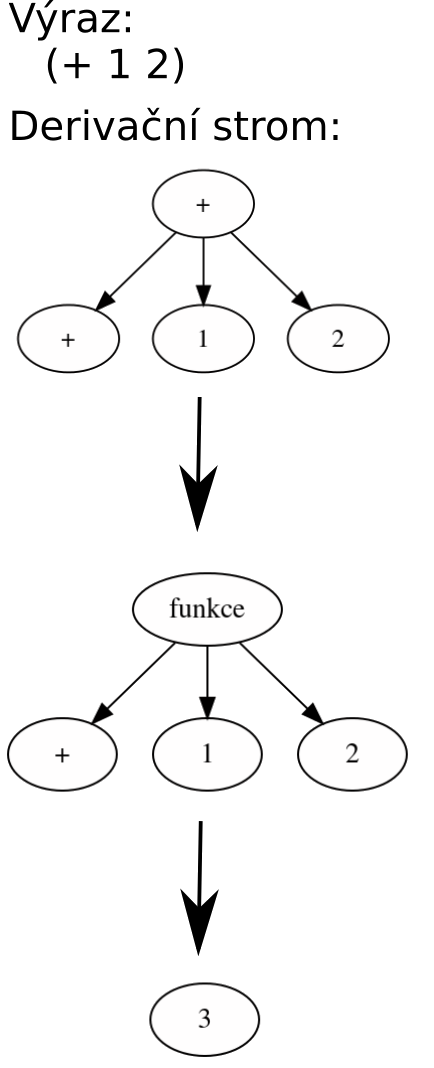
\includegraphics[width=0.4\textwidth]{obrazky/preklad.png}
    \caption{Vyhodnocení výrazu}
    \label{fig:Popis překladu}
\end{figure}
\newpage{}
\section{Spuštění a překlad}
Pro překlad je potřeba splnit následující závislosti:
\begin{enumerate}
\item Kompilátor s podporou c++ 14 (testováno na g++ 6.3.1, clang 3.8.1)
\item Nejnovější knihovnu boost \url{http://www.boost.org}
\item CMake 3.6 nebo vyšší
\end{enumerate}
Pro samotné sestavení je potřeba nejprve vygenerovat makefile (nebo Vámi zvolený target) s pomocí programu cmake a poté jej sestavit. Pro klasický makefile je posloupnost příkazů následující. Předpokládá se, že se nacházíte v kořenovém adresáři projektu.
\begin{lstlisting}[language=bash]
$ cmake -G "UnixMakefiles" CMakeLists.txt
$ make
\end{lstlisting}
Výsledkem kompilace jsou dva spustitelné soubory mirageI a mirageC. Soubor mirageI je interpreter, který načte řádek ze stdin, vyhodnotí ho a vytiskne výsledek na stdout. Soubor mirageC slouží k překladu samotných programů do svg. Může být buď zavolán s argumentem, který představuje název souboru, který se má načíst nebo bez argumentů, pak bude načítat ze stdin.

Pro správnou funkčnost všech příkladů je potřeba nastavit proměnnou prostředí MIRAGE\_PATH na cestu, která vede ke složce ve které se nachází standardní knihovna. Bez tohoto opatření by nebylo možné jí najít a tedy načíst. Alternativně je tu možnost hodit knihovnu k příkladům.
\end{document}